\documentclass[letterpaper,11pt,twoside,]{pinp}

%% Some pieces required from the pandoc template
\providecommand{\tightlist}{%
  \setlength{\itemsep}{0pt}\setlength{\parskip}{0pt}}

% Use the lineno option to display guide line numbers if required.
% Note that the use of elements such as single-column equations
% may affect the guide line number alignment.

\usepackage[T1]{fontenc}
\usepackage[utf8]{inputenc}
\usepackage{longtable}

% pinp change: the geometry package layout settings need to be set here, not in pinp.cls
\geometry{layoutsize={0.95588\paperwidth,0.98864\paperheight},%
  layouthoffset=0.02206\paperwidth, layoutvoffset=0.00568\paperheight}

\definecolor{pinpblue}{HTML}{185FAF}  % imagecolorpicker on blue for new R logo
\definecolor{pnasbluetext}{RGB}{101,0,0} %



\title{Lab 006 - Power Calculations - Solutions}

\author[a]{EPIB607 - Inferential Statistics}

  \affil[a]{McGill University}

\setcounter{secnumdepth}{5}

% Please give the surname of the lead author for the running footer
\leadauthor{Bhatnagar and Hanley}

% Keywords are not mandatory, but authors are strongly encouraged to provide them. If provided, please include two to five keywords, separated by the pipe symbol, e.g:
 

\begin{abstract}

\end{abstract}

\dates{This version was compiled on \today} 

% initially we use doi so keep for backwards compatibility
\doifooter{\url{https://sahirbhatnagar.com/EPIB607/}}
% new name is doi_footer

\pinpfootercontents{Lab 006}

\begin{document}

% Optional adjustment to line up main text (after abstract) of first page with line numbers, when using both lineno and twocolumn options.
% You should only change this length when you've finalised the article contents.
\verticaladjustment{-2pt}

\maketitle
\thispagestyle{firststyle}
\ifthenelse{\boolean{shortarticle}}{\ifthenelse{\boolean{singlecolumn}}{\abscontentformatted}{\abscontent}}{}

% If your first paragraph (i.e. with the \dropcap) contains a list environment (quote, quotation, theorem, definition, enumerate, itemize...), the line after the list may have some extra indentation. If this is the case, add \parshape=0 to the end of the list environment.


\begin{longtable}[]{@{}ll@{}}
\toprule
R Code & Value \\
\midrule
\endhead
\texttt{qnorm(p\ =\ c(0.05,\ 0.95))} & -1.64, 1.64 \\
\texttt{qnorm(p\ =\ c(0.025,\ 0.975))} & -1.96, 1.96 \\
\texttt{qnorm(p\ =\ c(0.005,\ 0.995))} & -2.58, 2.58 \\
\texttt{qt(p\ =\ c(0.025,\ 0.975),\ df\ =\ 400-1)} & -1.97, 1.97 \\
\texttt{qt(p\ =\ c(0.025,\ 0.975),\ df\ =\ 25-1)} & -2.06, 2.06 \\
\texttt{qt(p\ =\ c(0.025,\ 0.975),\ df\ =\ 20-1)} & -2.09, 2.09 \\
\texttt{qt(p\ =\ c(0.025,\ 0.975),\ df\ =\ 16-1)} & -2.13, 2.13 \\
\bottomrule
\end{longtable}

\hypertarget{lake-wobegon}{%
\section{Lake Wobegon}\label{lake-wobegon}}

It is claimed that the children of Lake Wobegon are above average. Take
a simple random sample of 9 children from Lake Wobegon, and measure
their IQ to obtain a sample mean of 112.8. IQ scores are scaled to be
Normally distributed with mean 100 and standard deviation 15.

\begin{enumerate}
\def\labelenumi{\alph{enumi})}
\tightlist
\item
  Does this sample provide evidence to reject the null hypothesis of no
  difference between children of Lake Wobegon and the general
  population?
\end{enumerate}

\[
H_0: \mu = 100 \qquad \qquad H_A: \mu > 100
\]

The p-value (one-sided test) is given by:

\begin{Shaded}
\begin{Highlighting}[]
\FunctionTok{pnorm}\NormalTok{(}\AttributeTok{q =} \FloatTok{112.8}\NormalTok{, }\AttributeTok{mean =} \DecValTok{100}\NormalTok{, }\AttributeTok{sd =} \DecValTok{15} \SpecialCharTok{/} \FunctionTok{sqrt}\NormalTok{(}\DecValTok{9}\NormalTok{), }\AttributeTok{lower.tail =} \ConstantTok{FALSE}\NormalTok{)}
\end{Highlighting}
\end{Shaded}

\begin{ShadedResult}
\begin{verbatim}
#  [1] 0.005233608
\end{verbatim}
\end{ShadedResult}

This sample provides evidence against the null hypothesis. We calculated
a p-value of 0.01 which tells us the probability of observing the sample
mean of 112.8 under the null hypothesis distribution is very unlikely.

\begin{enumerate}
\def\labelenumi{\alph{enumi})}
\setcounter{enumi}{1}
\tightlist
\item
  Suppose you hope to use a one-sided test to show that the children
  from Lake Wobegon are at least 10 points higher than average on the IQ
  test. What power do you have to detect this with the sample of 9
  children if using a 0.05-level test?
\end{enumerate}

\[
H_0: \mu = 100 \qquad \qquad H_A: \mu > 110
\]

Step 1 is to calculate the cutoff in order to reject the null. This is
given by

\begin{Shaded}
\begin{Highlighting}[]
\CommentTok{\# this is a one{-}sided alternative so we want alpha=5\% in the right tail}
\NormalTok{(cutoff }\OtherTok{\textless{}{-}} \FunctionTok{qnorm}\NormalTok{(}\AttributeTok{p =} \FloatTok{0.95}\NormalTok{, }\AttributeTok{mean =} \DecValTok{100}\NormalTok{, }\AttributeTok{sd =} \DecValTok{15} \SpecialCharTok{/} \FunctionTok{sqrt}\NormalTok{(}\DecValTok{9}\NormalTok{)))}
\end{Highlighting}
\end{Shaded}

\begin{ShadedResult}
\begin{verbatim}
#  [1] 108.2243
\end{verbatim}
\end{ShadedResult}

Then we calculate the probability of observing this cutoff or greater
under the alternative hypothesis:

\begin{Shaded}
\begin{Highlighting}[]
\FunctionTok{pnorm}\NormalTok{(}\AttributeTok{q =}\NormalTok{ cutoff, }\AttributeTok{mean =} \DecValTok{110}\NormalTok{, }\AttributeTok{sd =} \DecValTok{15} \SpecialCharTok{/} \FunctionTok{sqrt}\NormalTok{(}\DecValTok{9}\NormalTok{), }\AttributeTok{lower.tail =} \ConstantTok{FALSE}\NormalTok{)}
\end{Highlighting}
\end{Shaded}

\begin{ShadedResult}
\begin{verbatim}
#  [1] 0.63876
\end{verbatim}
\end{ShadedResult}

The following figure visualizes this calculation:

\begin{Shaded}
\begin{Highlighting}[]
\FunctionTok{source}\NormalTok{(}\StringTok{"https://raw.githubusercontent.com/sahirbhatnagar/EPIB607/master/inst/code/plot\_null\_alt.R"}\NormalTok{)}
\FunctionTok{power\_plot}\NormalTok{(}\AttributeTok{n =} \DecValTok{9}\NormalTok{, }\AttributeTok{s =} \DecValTok{15}\NormalTok{, }\AttributeTok{mu0 =} \DecValTok{100}\NormalTok{, }\AttributeTok{mha =} \DecValTok{110}\NormalTok{,}
           \AttributeTok{cutoff =} \FunctionTok{qnorm}\NormalTok{(}\AttributeTok{p =} \FloatTok{0.95}\NormalTok{, }\AttributeTok{mean =} \DecValTok{100}\NormalTok{, }\AttributeTok{sd =} \DecValTok{15} \SpecialCharTok{/} \FunctionTok{sqrt}\NormalTok{(}\DecValTok{9}\NormalTok{)),}
           \AttributeTok{alternative =} \StringTok{"greater"}\NormalTok{, }\AttributeTok{xlab =} \StringTok{"Average IQ Score"}\NormalTok{)}
\end{Highlighting}
\end{Shaded}

\begin{center}\includegraphics{006-power-solutions_files/figure-latex/unnamed-chunk-4-1} \end{center}

\begin{enumerate}
\def\labelenumi{\alph{enumi})}
\setcounter{enumi}{2}
\tightlist
\item
  If you hoped to use a \textbf{two-sided} test to show that the
  children from Lake Wobegon are at least 5 points higher than average
  on the IQ test, what power do you have with the sample size of 9 and a
  0.05-level test?
\end{enumerate}

\[
H_0: \mu = 100 \qquad \qquad H_A: \mu = 105
\]

Because its a two-sided test, we need to find the both cutoffs, i.e.,
the values of the sample mean that will reject the null. This is given
by:

\begin{Shaded}
\begin{Highlighting}[]
\CommentTok{\# two{-}sided test at alpha=5\% means we want 2.5\% in the tails}
\NormalTok{(cutoffs }\OtherTok{\textless{}{-}} \FunctionTok{qnorm}\NormalTok{(}\FunctionTok{c}\NormalTok{(}\FloatTok{0.025}\NormalTok{, }\FloatTok{0.975}\NormalTok{), }\DecValTok{100}\NormalTok{, }\DecValTok{15} \SpecialCharTok{/} \FunctionTok{sqrt}\NormalTok{(}\DecValTok{9}\NormalTok{)))}
\end{Highlighting}
\end{Shaded}

\begin{ShadedResult}
\begin{verbatim}
#  [1]  90.20018 109.79982
\end{verbatim}
\end{ShadedResult}

That is, we will reject the null hypothesis if the sample mean is 90.2
or less, OR reject than null if the sample mean is 109.8 or more.

Next we need to calculate these probabilities under the alternative
hypothesis:

\begin{Shaded}
\begin{Highlighting}[]
\CommentTok{\# left tail probability}
\NormalTok{(p\_left }\OtherTok{\textless{}{-}} \FunctionTok{pnorm}\NormalTok{(}\AttributeTok{q =} \FloatTok{90.20018}\NormalTok{, }\AttributeTok{mean =} \DecValTok{105}\NormalTok{, }\AttributeTok{sd =} \DecValTok{15} \SpecialCharTok{/} \FunctionTok{sqrt}\NormalTok{(}\DecValTok{9}\NormalTok{), }\AttributeTok{lower.tail =} \ConstantTok{TRUE}\NormalTok{))}
\end{Highlighting}
\end{Shaded}

\begin{ShadedResult}
\begin{verbatim}
#  [1] 0.001538375
\end{verbatim}
\end{ShadedResult}

\begin{Shaded}
\begin{Highlighting}[]
\CommentTok{\# right tail probability}
\NormalTok{(p\_right }\OtherTok{\textless{}{-}} \FunctionTok{pnorm}\NormalTok{(}\AttributeTok{q =} \FloatTok{109.79982}\NormalTok{, }\AttributeTok{mean =} \DecValTok{105}\NormalTok{, }\AttributeTok{sd =} \DecValTok{15} \SpecialCharTok{/} \FunctionTok{sqrt}\NormalTok{(}\DecValTok{9}\NormalTok{), }\AttributeTok{lower.tail =} \ConstantTok{FALSE}\NormalTok{))}
\end{Highlighting}
\end{Shaded}

\begin{ShadedResult}
\begin{verbatim}
#  [1] 0.1685367
\end{verbatim}
\end{ShadedResult}

And the power is the sum of these two probabilities:

\begin{Shaded}
\begin{Highlighting}[]
\NormalTok{p\_left }\SpecialCharTok{+}\NormalTok{ p\_right}
\end{Highlighting}
\end{Shaded}

\begin{ShadedResult}
\begin{verbatim}
#  [1] 0.170075
\end{verbatim}
\end{ShadedResult}

As show in the following figure:

\begin{Shaded}
\begin{Highlighting}[]
\FunctionTok{power\_plot}\NormalTok{(}\AttributeTok{n =} \DecValTok{9}\NormalTok{, }\AttributeTok{s =} \DecValTok{15}\NormalTok{, }\AttributeTok{mu0 =} \DecValTok{100}\NormalTok{, }\AttributeTok{mha =} \DecValTok{105}\NormalTok{,}
           \AttributeTok{cutoff =} \FunctionTok{qnorm}\NormalTok{(}\FunctionTok{c}\NormalTok{(}\FloatTok{0.025}\NormalTok{, }\FloatTok{0.975}\NormalTok{), }\DecValTok{100}\NormalTok{, }\DecValTok{15} \SpecialCharTok{/} \FunctionTok{sqrt}\NormalTok{(}\DecValTok{9}\NormalTok{)),}
           \AttributeTok{alternative =} \StringTok{"equal"}\NormalTok{, }\AttributeTok{xlab =} \StringTok{"Average IQ Score"}\NormalTok{)}
\end{Highlighting}
\end{Shaded}

\begin{center}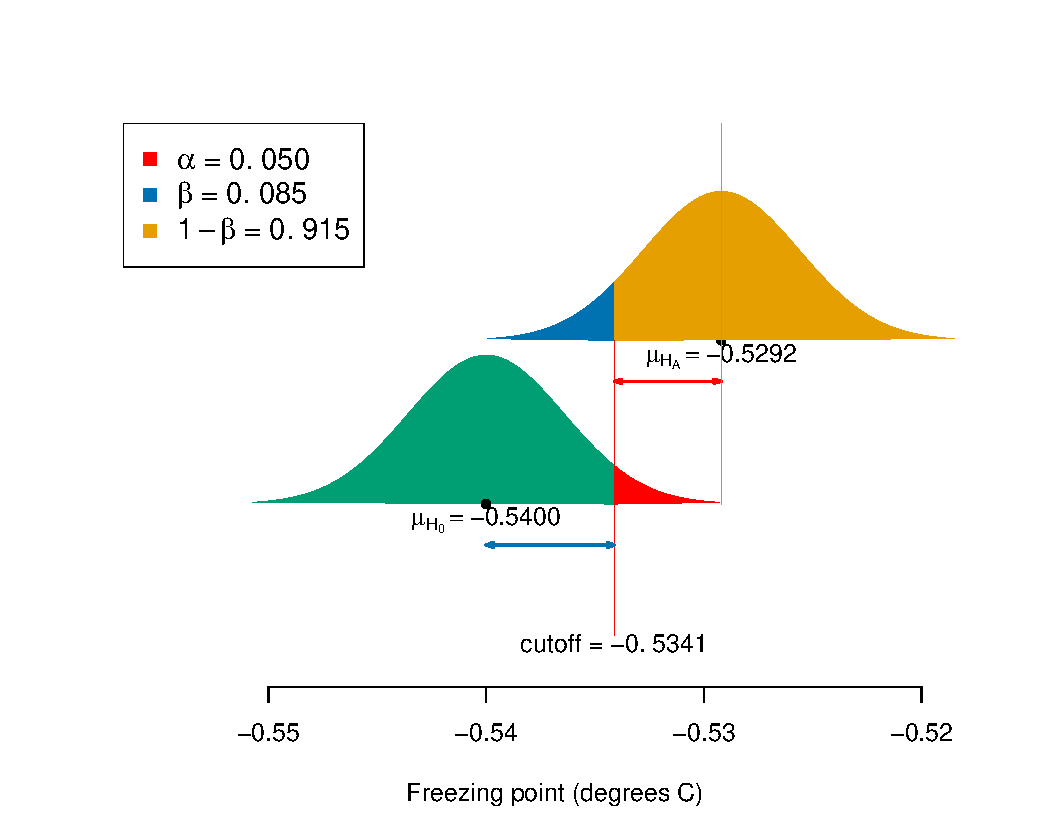
\includegraphics{006-power-solutions_files/figure-latex/unnamed-chunk-8-1} \end{center}

\hypertarget{bias-in-step-counters}{%
\section{Bias in step counters}\label{bias-in-step-counters}}

Following the study by
\href{http://www.medicine.mcgill.ca/epidemiology/hanley/bios601/Surveys/SmartphoneSteps.pdf}{Case
et al., JAMA, 2015}, suppose we wished to assess, via a formal
statistical test, whether (at an \textit{population}, rather than an
individual, level) a step-counting device or app is unbiased (\(H_0\))
or under-counts (\(H_A\)). Suppose we will do so the way
\href{http://www.medicine.mcgill.ca/epidemiology/hanley/bios601/Surveys/SmartphoneSteps.pdf}{Case
et al.} did, but measuring \(n\) persons just once each. We observe the
device count when the true count on the treadmill reaches 500.

\begin{enumerate}
\def\labelenumi{\alph{enumi}.}
\tightlist
\item
  Using a planned sample size of \(n=25\), and \(\sigma = 60\) steps as
  a pre-study best-guess as to the \(s\) that might be observed in them,
  calculate the critical value at \(\alpha = 0.01\).
\end{enumerate}

\begin{Shaded}
\begin{Highlighting}[]
\FunctionTok{qnorm}\NormalTok{(}\AttributeTok{p =} \FloatTok{0.01}\NormalTok{, }\AttributeTok{mean =} \DecValTok{500}\NormalTok{, }\AttributeTok{sd =} \DecValTok{60}\SpecialCharTok{/}\FunctionTok{sqrt}\NormalTok{(}\DecValTok{25}\NormalTok{))}
\end{Highlighting}
\end{Shaded}

\begin{ShadedResult}
\begin{verbatim}
#  [1] 472.0838
\end{verbatim}
\end{ShadedResult}

The critical value, i.e., the mean step counts to reject the null is
472.08 steps.

\begin{enumerate}
\def\labelenumi{\alph{enumi}.}
\setcounter{enumi}{1}
\tightlist
\item
  Now imagine that the mean would not be the null 500, but \(\mu=470.\)
  Calculate the probability that the mean in the sample of 25 will be
  less than this critical value. Use the same \(\sigma\) for the
  alternative that you used for the null. What is this probability
  called?
\end{enumerate}

\begin{Shaded}
\begin{Highlighting}[]
\NormalTok{critical\_z }\OtherTok{\textless{}{-}} \FunctionTok{qnorm}\NormalTok{(}\AttributeTok{p =} \FloatTok{0.01}\NormalTok{, }\AttributeTok{mean =} \DecValTok{500}\NormalTok{, }\AttributeTok{sd =} \DecValTok{60}\SpecialCharTok{/}\FunctionTok{sqrt}\NormalTok{(}\DecValTok{25}\NormalTok{))}
\FunctionTok{pnorm}\NormalTok{(}\AttributeTok{q =}\NormalTok{ critical\_z, }\AttributeTok{mean =} \DecValTok{470}\NormalTok{, }\AttributeTok{sd =} \DecValTok{60}\SpecialCharTok{/}\FunctionTok{sqrt}\NormalTok{(}\DecValTok{25}\NormalTok{), }\AttributeTok{lower.tail =} \ConstantTok{TRUE}\NormalTok{)}
\end{Highlighting}
\end{Shaded}

\begin{ShadedResult}
\begin{verbatim}
#  [1] 0.5689306
\end{verbatim}
\end{ShadedResult}

The probability of getting a sample of size 25 with a mean less than the
critical value of 472.08 steps is 0.5689306. This is the statistical
power to detect a mean difference of 30 fewer steps.

\begin{Shaded}
\begin{Highlighting}[]
\FunctionTok{power\_plot}\NormalTok{(}\AttributeTok{n =} \DecValTok{25}\NormalTok{, }\AttributeTok{s =} \DecValTok{60}\NormalTok{, }\AttributeTok{mu0 =} \DecValTok{500}\NormalTok{, }\AttributeTok{mha =} \DecValTok{470}\NormalTok{,}
           \AttributeTok{cutoff =}\NormalTok{ critical\_z,}
           \AttributeTok{alternative =} \StringTok{"less"}\NormalTok{, }\AttributeTok{xlab =} \StringTok{"Mean number of steps"}\NormalTok{)}
\end{Highlighting}
\end{Shaded}

\begin{center}\includegraphics{006-power-solutions_files/figure-latex/unnamed-chunk-11-1} \end{center}

\begin{enumerate}
\def\labelenumi{\alph{enumi}.}
\setcounter{enumi}{2}
\tightlist
\item
  Determine the sample size required to detect a 30 step mean decrease
  in steps with 80\% power using a 1\% level of significance. Plot the
  null and alternative distributions in a diagram using the
  \href{https://raw.githubusercontent.com/sahirbhatnagar/EPIB607/master/inst/code/plot_null_alt.R}{\texttt{plot\_power}}
  function.
\end{enumerate}

Under the null hypothesis, we know that the mean step count has to be
2.32 standard errors of the mean away from \(\mu_0=500\) in order to
reject the null hypothesis at an \(\alpha=0.01\). 2.32 is the \(z\)
value such that there is 0.01 area in the left tail of the null
distribution:

\begin{Shaded}
\begin{Highlighting}[]
\FunctionTok{qnorm}\NormalTok{(}\AttributeTok{p =} \FloatTok{0.01}\NormalTok{, }\AttributeTok{lower.tail =} \ConstantTok{TRUE}\NormalTok{)}
\end{Highlighting}
\end{Shaded}

\begin{ShadedResult}
\begin{verbatim}
#  [1] -2.326348
\end{verbatim}
\end{ShadedResult}

Under the alternative hypothesis, we know that the mean step count has
to be 0.84 standard errors of the mean (SEM) away from \(\mu_A=470\)
such that there is 20\% area in the right tail of the alternative
hypothesis distribution:

\begin{Shaded}
\begin{Highlighting}[]
\FunctionTok{qnorm}\NormalTok{(}\AttributeTok{p =} \FloatTok{0.20}\NormalTok{, }\AttributeTok{lower.tail =} \ConstantTok{FALSE}\NormalTok{)}
\end{Highlighting}
\end{Shaded}

\begin{ShadedResult}
\begin{verbatim}
#  [1] 0.8416212
\end{verbatim}
\end{ShadedResult}

We know that the distance between \(\mu_0=500\) and \(\mu_A=470\) must
be equal to 0.84SEM + 2.32SEM. Note that although the quantile
calculated under the null is negative, since we are dealing with
distance, we use the absolute value. This is the balancing equation:

\begin{align*}
\Delta &= 0.84\times SEM + 2.32\times SEM \\
\Delta &= (0.84 + 2.32) SEM \\
 &= (0.84 + 2.32) \frac{\sigma}{\sqrt{n}} \\
\sqrt{n} & = (0.84 + 2.32) \frac{\sigma}{\Delta}\\
n & = (0.84 + 2.32)^2 \left(\frac{\sigma}{\Delta}\right)^2 \\
 & = (0.84 + 2.32)^2 \left(\frac{60}{30}\right)^2 \\
 & = 40.14
\end{align*}

Therefore we need 41 subjects to detect a 30 step mean decrease in steps
with 80\% power using a 1\% level of significance.

\begin{Shaded}
\begin{Highlighting}[]
\FunctionTok{source}\NormalTok{(}\StringTok{"https://raw.githubusercontent.com/sahirbhatnagar/EPIB607/master/inst/code/plot\_null\_alt.R"}\NormalTok{)}

\FunctionTok{power\_plot}\NormalTok{(}\AttributeTok{n =} \DecValTok{41}\NormalTok{,}
           \AttributeTok{s =} \DecValTok{60}\NormalTok{,}
           \AttributeTok{mu0 =} \DecValTok{500}\NormalTok{,}
           \AttributeTok{mha =} \DecValTok{470}\NormalTok{,}
           \AttributeTok{cutoff =} \FunctionTok{qnorm}\NormalTok{(}\FloatTok{0.01}\NormalTok{, }\AttributeTok{mean =} \DecValTok{500}\NormalTok{, }\AttributeTok{sd=} \DecValTok{60}\SpecialCharTok{/}\FunctionTok{sqrt}\NormalTok{(}\DecValTok{41}\NormalTok{), }\AttributeTok{lower.tail =} \ConstantTok{TRUE}\NormalTok{),}
           \AttributeTok{alternative =} \StringTok{"less"}\NormalTok{,}
           \AttributeTok{xlab =} \StringTok{"Mean number of steps "}\NormalTok{)}
\end{Highlighting}
\end{Shaded}

\begin{center}\includegraphics{006-power-solutions_files/figure-latex/unnamed-chunk-14-1} \end{center}

%\showmatmethods


\bibliography{pinp}
\bibliographystyle{jss}



\end{document}
